% Este arquivo .tex será incluído no arquivo .tex principal. Não é preciso
% declarar nenhum cabeçalho

\section{Grupos e Entidades da Unicamp}

\subsection{Alumni Computação Unicamp}

\begin{figure}[H]
    \centering
    
\includegraphics[scale=0.40]{img/alumni_comp.png}
\end{figure}

Alumni é o nome dado a ex-alunos de uma universidade. Por extensão,
alumni também é o nome de organizações sem fins lucrativos motivadas em manter
o relacionamento entre a universidade e os ex-alunos e o destes entre si, servindo como uma rede
de contatos profissionais. A comunicação entre alunos, ex-alunos e professores proporciona um compartilhamento de experiência e informações, que contribuem para uma diferenciação acadêmica, cultural e profissional.

O \textbf{Alumni Computação Unicamp} é uma forma de manter todos que passaram
pelo melhor curso de computação da América Latina conectados -- tanto alunos
quanto ex-alunos. Atualmente o Alumni conta com uma página no Facebook (\url{fb.com/AlumniComputacaoUnicamp}), que reúne os grupos das turmas que passaram pela Computação, com o objetivo de atingir o maior número de alunos e ex-alunos.

Participe do grupo de sua turma, convide seus amigos a curtirem a página, envie sugestões e contribua para essa ideia!

\subsection{ARU}

\subsubsection{O que é a ARU – Associação de Repúblicas da Unicamp?}

\begin{figure}[H]
    \centering
    
\includegraphics[scale=0.40]{img/aru.png}
\end{figure}

Idealizada em 2008, a ARU é a entidade que representa as Repúblicas Associadas de
Barão Geraldo.  Tem como meta prestar apoio a elas, zelar pela sua segurança
e bem estar com toda a vizinhança, como também servir de espaço
para discutir os problemas apresentados em reuniões.

\begin{figure}[H]
    \centering
    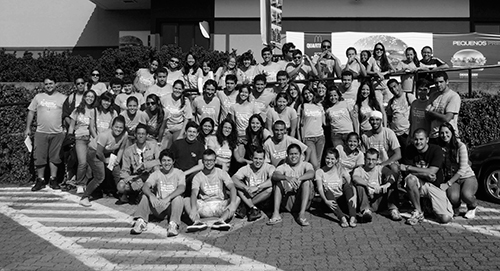
\includegraphics[scale=0.40]{img/aru_foto.jpg}
\end{figure}

Além de entregar no começo do ano um manual para os bixos contendo informações
sobre as Repúblicas Associadas, a ARU também realiza vários eventos, os quais
têm o objetivo de integrar e divertir os moradores de repúblicas. Alguns deles
são: a \textbf{Alcorrida}, a \textbf{Campanha do Agasalho},
o \textbf{EntortaRep}, e, principalmente, o \textbf{InterReps}.

\subsubsection{Contato}

\begin{itemize}
    \item Site: \url{www.republicasunicamp.com.br}
    \item E-mail: \url{contato@republicasunicamp.com.br}
    \item Facebook: \url{fb.com/republicasunicamp}
\end{itemize}

\subsection{Competições de programação}

Curte programar? Nunca programou mas está gostando de MC102? Já brincou de
Olimpíada naquelas provas com direito a medalha? Vá fundo! Para os bixos
com menos de 20 anos existe a \textbf{OBI -- Olimpíada Brasileira de Informática}, logo no primeiro
semestre. Anualmente, muitos alunos do IC, tanto da Ciência como da Engenharia, ganham premiações
nessa competição. O site dela é \url{olimpiada.ic.unicamp.br}. Esteja
sempre visitando-o.

\begin{figure}[h!]
    \centering
    
\includegraphics[scale=0.40, keepaspectratio=true]{img/maratona.png}
\end{figure}

A OBI serve como familiarização para outra competição -- a Maratona de Programação, que consiste de
problemas mais difíceis e é feita
em equipes de três alunos. A Unicamp tem grande tradição nessa competição,
tendo sido campeã da regional brasileira em
2000, 2002 e 2004. Já houve campeões da Ciência, do mestrado, das duas
modalidades da Engenharia, além de bixos medalhistas. Para maiores informações,
acesse o site da organização nacional: \url{maratona.ime.usp.br}.

Para participar dos treinamentos para a Maratona que acontecem na Unicamp,
inscreva-se no grupo \url{groups.google.com/group/maratona_unicamp}.

\subsection{DCE}

Criado em 1978, o DCE Unicamp (Diretório Central dos Estudantes) é a entidade que
representa todos os estudantes de graduação da Universidade, articulando
e organizando o movimento estudantil (ME).

Cabe ao DCE representar o conjunto dos
estudantes em todos os espaços dentro e fora da universidade, diante das mais
diversas entidades (reitoria, sindicatos, DCEs de outras universidades, centros
acadêmicos, associações etc.) e movimentos sociais.

Como articulador do ME, cabe ao DCE organizar os estudantes na luta por uma
educação superior realmente pública, gratuita e de qualidade. Para tanto,
é papel fundamental do DCE propor, juntamente com os centros acadêmicos,
discussões políticas que extrapolem os nossos currículos e o nosso dia a dia.
Além disso, o DCE deve propor ações que vão ao encontro das reivindicações
estudantis, de forma que elas sejam levadas e cobradas da reitoria ou até mesmo
do governo.

O DCE esteve envolvido em várias conquistas dos estudantes, das quais se
destacam algumas lutas históricas: a construção da moradia estudantil; a melhoria
de estrutura para cursos noturnos, que tornou acessível para esse período
bibliotecas, xérox, laboratórios e secretarias de graduação; a reunião semestral
para avaliação de curso; o não-aumento do preço do bandejão; uma seleção mais
justa para as vagas na moradia; entre diversas outras. Além disso, o DCE teve
participação em importantes lutas sociais que extrapolam o âmbito da Unicamp,
como a organização do Plebiscito contra a Alca e do Plebiscito contra o Provão;
a luta por mais verbas para a educação no estado de São Paulo; diversas lutas
pela qualidade do ensino e manutenção de direitos dos estudantes em outras
universidades como na UNIP, UNIMEP, FUPPESP etc.

No fim do ano, há eleições para definir qual
a chapa que comandará a entidade no ano seguinte, juntamente com eleições para
representação discente no Consu e na CCG. É muito importante a participação dos
alunos nessas eleições.

Não deixe de participar da Calourada Integrada organizada pelo DCE e centros
acadêmicos e das reuniões do DCE, que acontecem na sede próxima ao Bandejão.

\begin{itemize}
\item  Telefones: (19) 3521-7910, (19) 3521-7042.
\item  E-mail: \url{dceunicamp@gmail.com}.
\item  Site: \url{dceunicamp.org.br}.
\end{itemize}

\subsection{Gamux}

O Gamux (Grupo de Pesquisa e Desenvolvimento de Jogos da Unicamp), composto por
computeiros e alunos do IA (Instituto de Artes), é uma ótima oportunidade para
quem tiver curiosidade de saber como são feitos os jogos eletrônicos.

Fique atento, eles costumam organizar ciclos de palestras e eventos relacionados
a desenvolvimento de jogos.

Mas não precisa esperar até lá! Apareça no LMS (Laboratório da Microsoft,
próximo as mesinhas do IC3) ou entre no grupo de e-mail.

\begin{itemize}
\item  Site: \url{gamux.com.br}
\item  Lista de discussão: \url{groups.google.com/group/gamedev_unicamp}
\end{itemize}

\subsection{GPSL}

O Grupo Pró Software Livre (GPSL) é aberto para alunos de todos os institutos
e para a comunidade. Seu objetivo é promover o uso e o desenvolvimento do
software livre.

A maioria das instituições educacionais utiliza apenas software
proprietário e a Unicamp não é exceção. São poucos os institutos que usam
software livre e é muito fácil se formar sem sequer saber da existência ou ter
qualquer experiência com algo diferente do software proprietário vigente.

\begin{figure}[h!]
    \centering
    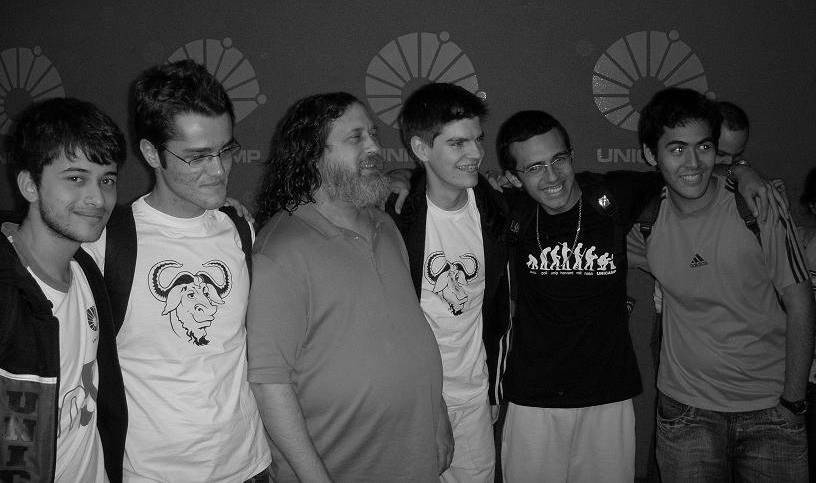
\includegraphics[scale=0.36, keepaspectratio=true]{img/imgs/18-grupos_entidades/stallman2.JPG}
    \caption{Richard Stallman em vista à Unicamp}
\end{figure}

O GPSL é um espaço para refletir sobre este monopólio do software proprietário,
imposto sobre nós através de tantas instâncias, inclusive nossa própria
universidade, a ética (ou falta de ética) por trás disso e seus efeitos sociais.
É também um espaço para se articular e pensar em formas de ação, que podem
envolver desde a educação e conscientização dos usuários de computadores até
o próprio desenvolvimento de software livre. O GPSL também pensa sobre
questões de mercado e econômicas relacionadas ao software livre.

Ultimamente, o GPSL tem sido responsável por organizar, com o apoio do
CACo, o \textbf{Curso de GNU/Linux para os bixos}. Este curso, como o
próprio nome diz, é voltado para os bixos que ingressam nos cursos de
Ciência e Engenharia da Computação (apesar de também ser aberto a todos
os outros alunos dos dois cursos), e tem como objetivo ensinar o
básico do sistema operacional \texttt{GNU/Linux} para você se virar
nas matérias de computação do primeiro semestre. Ele geralmente é
ministrado em abril, mas não existe data fixa. Mas não se preocupe,
algum veterano seu vai passar na sala de aula avisando sobre o curso,
além de sempre avisarmos com antecedência enviando um comunicado ao
seu e-mail do IC.

Para entrar no nossa lista de discussão mande um e-mail para
gpsl-unicamp@googlegroups.com, ou então se cadastre através do site:
\url{groups.google.com/group/gpsl-unicamp}.

\subsection{MTE}

O \textbf{MTE -- Mercado de Trabalho em Engenharia} é uma entidade estudantil que visa colocar o aluno da Unicamp em
contato mais próximo com o mercado de trabalho e com as possibilidades que ele
proporciona, mostrando as diferentes áreas de atuação de um engenheiro.

A participação no MTE desenvolve habilidades como networking, oratória, expressão, empreendedorismo, gestão e diversas outras.

A estrutura do MTE é dividida em três pilares:

\begin{itemize}
\item Oportunidades: responsável por atividades como visitas técnicas e captação de treinamentos e palestras.
\item Desenvolvimento: responsável por atividades como English Meeting (encontros de conversação em inglês), Teia do Conhecimento (treinamentos dados por algum dos membros) e Ciclo de Oratória (ciclos com foco em melhoria de expressão).
\item Orientação e Carreira: responsável pela estruturação pessoal e profissional dos membros realizando feedbacks, atividades de consultoria, de motivação, entrevista com profissionais e confraternizações.
\end{itemize}

Além da participação em um dos pilares, alguns membros participam da diretoria administrativo-financeira e, para completar, participam da realização de dois principais eventos: o EMC (Estudante e Mercado Conectados) que conta com visitas técnicas e palestras e o ArenaMTE, um desafio universitário de resolução de cases.

Para mais informações sobre o MTE e seu processo seletivo, acesse
\url{mte.org.br}.

\subsection{Rádio Muda}

Você provavelmente nunca viu nada do tipo na sua vida. Uma rádio na qual
qualquer ser humano pode fazer o seu programa tranquilamente, sem burocracias
(tendo espaço na grade de horários, lógico).

A Rádio Muda fica embaixo da caixa d'água (carinhosamente apelidada de Pau do
Zeferino) que fica perto do Teatro de Arena, bem em frente à BC (Biblioteca
Central).

Se você só quiser ouvir a muda, 88,5 MHz no seu rádio (em Barão Geraldo ou
Paulínia) ou pela Internet, através do site \url{muda.radiolivre.org}.

\subsection{Curso Exato}

O Curso Exato é um projeto da Pró-Reitoria de Extensão e Assuntos Comunitários
da Unicamp criado em 2008 por alunos de graduação, com a finalidade de explorar
o potencial e a capacidade dos alunos de se expressarem, de raciocinarem
logicamente e de compreenderem o mundo que os cerca, por meio de aulas de Língua
Portuguesa, Matemática, Física e Química.

Os professores do curso são alunos de graduação e pós-graduação da universidade
e o público alvo é constituído por alunos da rede pública de ensino com
disposição e interesse para aprender.

As aulas são realizadas no período noturno, das 19h15 às 22h30, de segunda
a quinta-feira, no campus da universidade.

\begin{itemize}
\item Site: \url{www.cursoexato.com.br}
\item Facebook: \url{facebook.com/curso.exato}
\item E-mail pra contato: \url{curso.exato@gmail.com}
\end{itemize}

\subsection{Grupos Religiosos}

\subsubsection{ABU -- Aliança Bíblica Universitária}

Grupo evangélico não ligado a nenhuma denominação, organiza várias reuniões
e grupos de discussões e é filiado à Aliança Bíblica Universitária do Brasil
(\url{www.abub.org.br}). Quaisquer dúvidas, entre no site
\url{www.abucampinas.org}, mande um e-mail para contato [@] abucampinas
[.] org ou abucamp\_co [@] yahoogrupos [.] com [.] br ou ainda ligue para (19)
3289-2823.

\subsubsection{Pastoral Universitária}

Grupo católico que se reúne semanalmente para estudar textos (bíblicos ou não),
livros, documentos, aprofundar a fé e promover a integração e união de seus
participantes. A Pastoral Universitária também organiza grupos de preparação
para Primeira Comunhão e Crisma, além de duas Missas semanais e Grupos de Oração
Universitários (GOUs). As Missas são realizadas às terças (18h) e às
quintas (12h15), sempre no PB04. Os GOUs acontecem às terças (12h15) e
nas quintas (18h), também no PB04. Quaisquer dúvidas, acesse o site da
Pastoral (\url{sites.google.com/site/pastoralunicamp/}) ou
envie um e-mail para pastoralunicamp [@] gmail [.] com.

\newpage
\section{Conpec}

\begin{figure}[H]
    \centering
    
\includegraphics[scale=0.40]{img/conpec.png}
\end{figure}

A Conpec é a empresa júnior dos cursos de Ciência e Engenharia de Computação da
Unicamp.

Nela você tem a oportunidade de aplicar os conhecimentos teóricos
adquiridos em sua vida acadêmica em uma situação real, de mercado, com clientes,
prazos e soluções reais. É uma chance ainda de aprender sobre aspectos de mercado de trabalho que você
nunca veria na faculdade, como marketing, finanças, planejamento, trabalho em equipe e liderança,
indispensáveis considerando-se que o perfil empreendedor é cada vez mais exigido do profissional de
computação. Muitos membros e ex-membros da Conpec usam os
conhecimentos adquiridos na empresa não só como um adicional ao buscar uma vaga
no mercado de trabalho, mas também para montar suas próprias empresas ou em
serviços não ligados diretamente à computação, como consultorias estratégicas.

Além disso, a Conpec é uma excelente oportunidade para conhecer os seus colegas
de curso, sejam veteranos ou bixos, pessoas de outros cursos e até mesmo de fora da
Unicamp, uma vez que há diversas empresas juniores espalhadas pelas universidades de São Paulo e do Brasil. É ainda uma grande chance para perder a inibição de falar em
público e aperfeiçoar sua capacidade de expor opiniões, além de aprender como
agir em um ambiente profissional.

\begin{figure}[H]
    \centering
    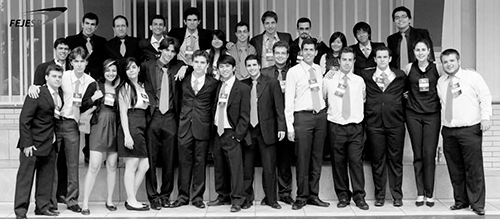
\includegraphics[scale=0.40]{img/conpec_foto.jpg}
\end{figure}

Para fazer parte da Conpec, fique atento à data da palestra de apresentação do
processo seletivo, que ocorre no início do ano.

Para saber mais sobre a empresa visite o site \url{conpec.com.br} ou
tire suas dúvidas mandando um e-mail para \url{conpec@conpec.com.br}.

\newpage
\section{Atlética -- AAACEC}

Assim como em outras unidades de ensino da Unicamp, o Instituto de Computação
(IC) e a Faculdade de Engenharia Elétrica e de Computação (FEEC) tem sua
entidade que promove a prática de eventos desportivos entre os membros da
graduação e da pós-graduação: A Associação Atlética Acadêmica da Ciência
e Engenharia da Computação, mais conhecida como AAACEC, ou simplesmente
\textbf{Atlética}. A AAACEC é uma entidade sem fins lucrativos, que tem uma
diretoria composta por alunos da computação, eleita a cada ano pelos alunos
dos cursos de Engenharia e Ciência da Computação e pós-graduandos vinculados ao IC.

A AAACEC é a entidade responsável pela participação da Computação em competições
esportivas, tanto dentro da Unicamp (Calouríadas, Interanos, Olimpíadas) como
com faculdades de outras cidades (Intercomp),
\begin{figure}[h!]
    \vspace{-10pt}
    \centering
    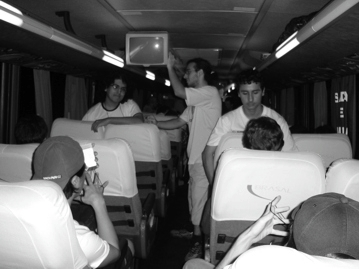
\includegraphics[scale=0.75, keepaspectratio=true]{img/imgs/20-aaacec/-096.jpg}
    \vspace{-10pt}
\end{figure}
competições essas que costumam
acontecer uma vez a cada ano. A fim de possibilitar essa participação, a AAACEC,
além de se encarregar das inscrições e organização, promove treinos regulares de
basquete, vôlei, handball e futsal, e disponibiliza o material (bolas, redes,
etc.) para a prática de tais esportes. A AAACEC se encarrega da reserva e/ou
locação de quadras para a realização dos treinos e competições em que isso se
fizer necessário. Os treinos são semanais e oferecidos para as modalidades
masculina e feminina, de forma que qualquer associado da Atlética pode
participar.

\subsection{Como, então, se associar à AAACEC?}

No caso dos recém-ingressantes, o jeito mais simples é comprando o KIT BIXO,
organizado pela própria AAACEC, contendo camiseta, caneca e outros produtos da
Atlética. Com ele, o calouro torna-se sócio e pode usufruir livremente de todos
os jogos e/ou eventos que a AAACEC venha a organizar pelo resto de sua vida.

Quem não comprar o Kit Bixo no primeiro ano, pode se associar mais tarde com o
pagamento de uma taxa de associação. Além do Kit Bixo, a AAACEC tem diversos
produtos que podem ser comprados por qualquer associado durante todo o curso,
como camisetas, blusas, agasalhos, adesivos, chaveiros, mouse-pads, entre
outros.

\subsection{E para quem vai o dinheiro da compra do kit bixo e dos demais produtos?}

A AAACEC promove a integração entre os alunos, e a realização de experiências
sociais e esportivas:

\begin{itemize}
\item  \textbf{A famosa Choppada Comp/Enf} (gratuita para os bixos)
\item  \textbf{Churrascos}
\item  \textbf{Torneios Esportivos:}
\begin{itemize}
\item  \textit{Internos} (Torneio início, Calouríadas, InterAnos, Olimpíadas)
\item  \textit{Externos} (Intercomp, UniSinos)
\end{itemize}
\begin{figure}[h!]
    \vspace{-10pt}
    \centering
    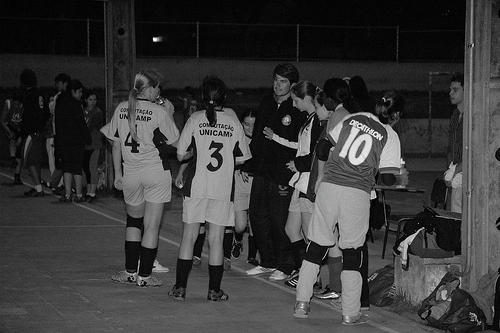
\includegraphics[scale=0.58, keepaspectratio=true]{img/imgs/20-aaacec/-100.jpg}
    \vspace{-10pt}
\end{figure}
\item  \textbf{Festas} (Muitas delas em união com outros cursos, promovendo ainda maior integração)
\end{itemize}

Para tudo isso, é necessário capital, que é obtido com muito trabalho da
Diretoria com a venda dos Kits Bixo e produtos.

É importante lembrar que a diretoria não tem remuneração alguma: Os diretores
trabalham pelo ideal comum de fazer a Computação crescer, e, consequentemente,
ganhar experiência de organização de eventos e pessoas, aprendizado de valor
inestimável, tanto na vida profissional como social.

A AAACEC busca fortalecer, acima de tudo, o nome do curso de Computação da
Unicamp, enaltecendo nossas qualidades dentro e fora da Universidade! Orgulho de
ser Computação Unicamp!!

Faça parte você também dessa integração! Associe-se à AAACEC!

As diretorias anteriores da AAACEC podem ser vistas em:
\url{aaacec.com/diretoria}

\subsection{Contato}

Não hesite em tirar dúvidas ou enviar sugestões!

\begin{itemize}
\item  E-mail: aaacec@ic.unicamp.br
\item  Site: \url{aaacec.com}
\end{itemize}

\subsection{Atendimento}

Ainda não há uma definição para este semestre, mas provavelmente o atendimento
será de segunda a sexta das 12h30m às 13h30m e segunda a quinta das 18h-19h

\subsection{Reuniões}

As reuniões serão marcadas no começo do semestre. Elas são realizadas num dia
letivo às 12h no IC-3.

\subsection{Bateria Valorosa}

Criada em 1998, a bateria Valorosa é umas das melhores baterias da Unicamp.

Durante o ano, ela participa de diversos eventos, como o Intercomp, Interbatuc,
UPA, e apoiando nossos atletas em jogos internos. Também somos convidados por
outros cursos para tocar em seus jogos.

A Bateria realiza ensaios semanais, dos quais estão todos convidados a
participar.

Esperamos que muitos bixos participem, e para isso basta comparecer aos ensaios,
lembrando que não é necessário saber tocar nenhum instrumento. TODOS que
quiserem aprender serão muito bem-vindos na bateria!

\twocolumn
\section{CACo -- Centro Acadêmico da Computação}

\begin{figure}[H]
    \centering
    
\includegraphics[scale=0.37]{img/caco/logo.png}
\end{figure}

Bixo, o CACo é o seu centro acadêmico. Um CA é uma entidade estudantil que, em
linhas gerais, deve trabalhar para garantir os interesses dos estudantes e
melhorar o curso e a faculdade a que pertence. O CACo é formado pelos alunos
de graduação tanto em Engenharia quanto em Ciência da Computação da Unicamp,
bem como os alunos de pós-graduação do IC. Todo e qualquer aluno desses cursos
é membro do CACo e isso inclui você.

Um centro acadêmico é parte do famoso ``movimento estudantil'' de que você
provavelmente já ouviu falar. Mas não se engane! Pergunte para o seu pai o que ele
pensa quando lê ``movimento estudantil'' e ele vai dizer que vê um bando de
estudantes desocupados associados a um partido político de esquerda que saem por
aí protestando contra o sistema e queimando ônibus pelas ruas. Se você pensa
assim, mude sua ideia: o CACo não é nada disso.

\begin{figure}[H]
    \centering
    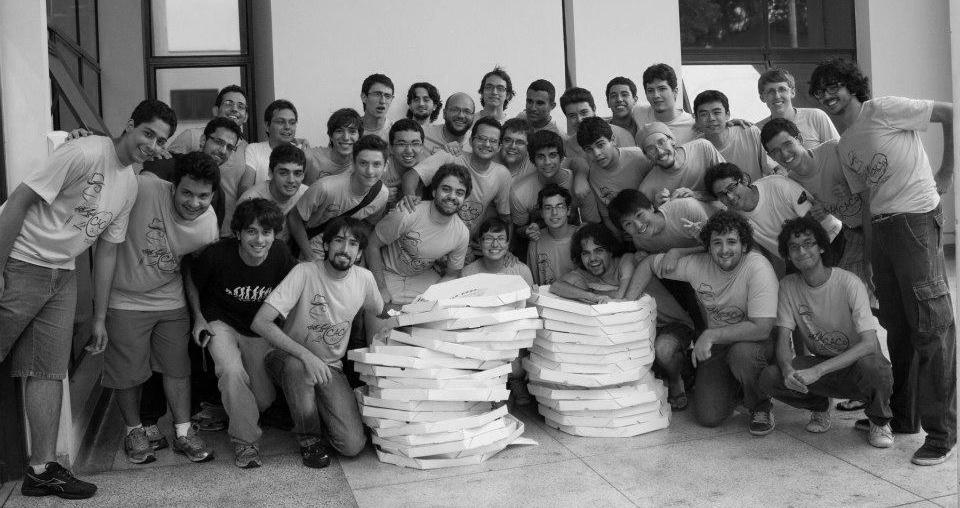
\includegraphics[scale=0.22]{img/caco/pizzada.jpg}
\end{figure}

O CACo tem como função representar os estudantes no âmbito acadêmico, ou seja,
perante o IC, a FEEC e a Unicamp. Mas o que o CACo faz? De forma
simplificada, procuramos ser porta-voz dos alunos. Reivindicamos espaço físico
decente para os alunos, alteração nas matérias e professores, promovemos
discussões sobre temas polêmicos e delicados, dentre muitas outras atividades.

Quer um exemplo? Esse estupendo manual que você está lendo neste exato momento
foi confeccionado pelo seu centro acadêmico para lhe ajudar no início da sua
vida universitária e, na verdade, você ainda vai se pegar recorrendo ao seu
Manual várias vezes durante seus quatro, cinco, doze anos na Unicamp.

Uma grande função do CACo é prezar pela qualidade dos cursos e fazemos isso, por
exemplo, através de discussões com o próprio Instituto, onde levamos reclamações
e reivindicações dos alunos para os coordenadores e professores.

\begin{figure}[H]
    \centering
    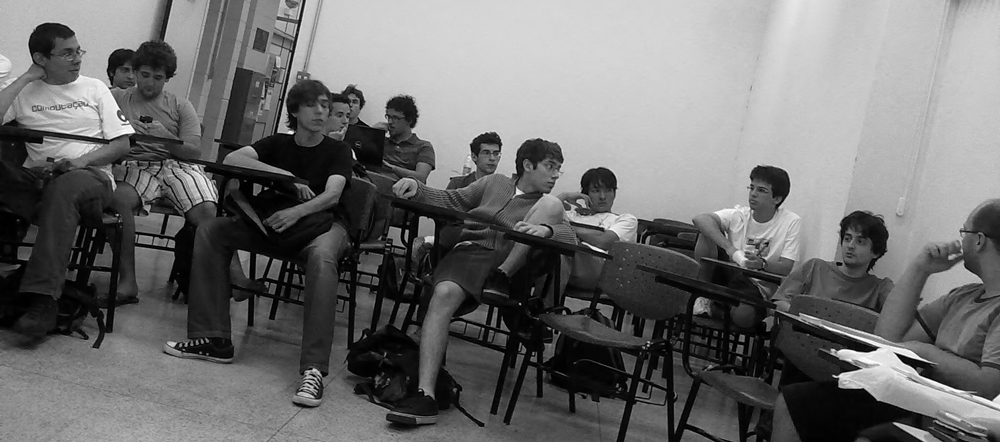
\includegraphics[scale=0.21]{img/caco/reuniao.jpg}
\end{figure}

Uma outra função do CACo é integrar os estudantes de computação da Unicamp. Para
isso, realizamos diversos eventos como o CineCACo, o PipoCACo, o CACo Games, o
CACo Series of Poker e a grande comemoração do Aniversário do CACo, que contou
com pizza de graça para mais de duzentos alunos! Tentamos também facilitar a
vida da galera através dos armários que alugamos, o Banco de Livros, o Banco de
Provas (o maior da Unicamp) e a máquina de café que colocamos no IC.

Repetindo o que foi dito antes: bixo, o CACo é o \textbf{seu} Centro Acadêmico.
Tudo que dissemos que fazemos pelos alunos, queremos fazer por você também. Por
isso, quando houver algum problema envolvendo a FEEC, o IC, os professores ou
qualquer coisa do tipo, não hesite em nos procurar. O CACo sempre lhe dará todo
o suporte necessário. Se tiver reclamação ou sugestão relacionada ao próprio
CACo, também estaremos aqui para ouvir. Mais do que isso, venha participar de
uma de nossas reuniões, que são abertas a você e todos os alunos de computação
da Unicamp.

\begin{figure}[H]
    \centering
    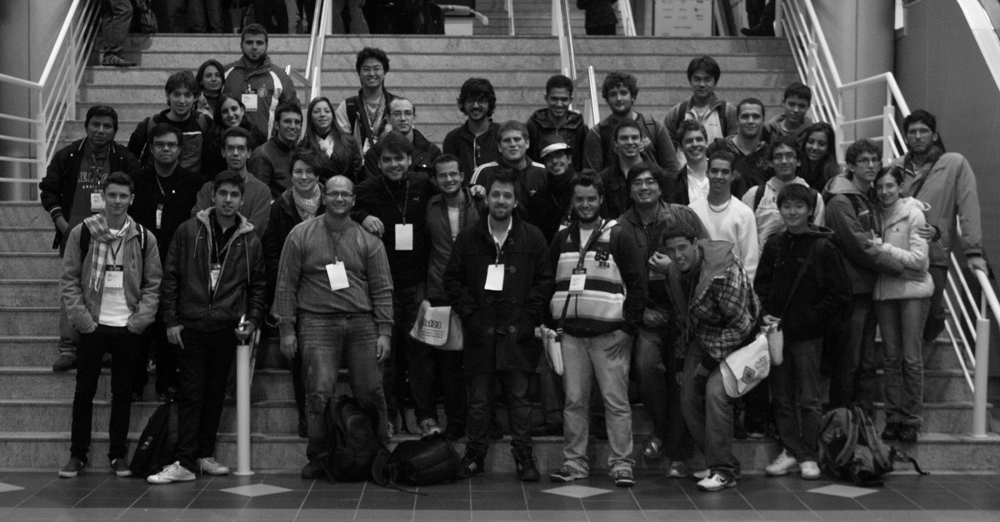
\includegraphics[scale=0.21]{img/caco/fisl2.jpg}
\end{figure}

Participar do CACo é uma experiência diferente de tudo aquilo que você terá na
sua graduação. É a chance de aprender e crescer de uma forma que não acontece em
nenhuma aula de cálculo. É uma oportunidade de conhecer seus veteranos e também
seus amiguinhos bixos. Mas, acima de tudo, é uma experiência pessoal onde você
vai aprender a se expressar, argumentar, defender suas ideias, falar em público
e pensar no coletivo. Você entrará em contato com muita gente que provavelmente
você nunca iria conhecer e, com certeza, fará amizade com muitos deles. Por
esses e muitos outros motivos é que você, bixo, deve vir a pelo menos uma
reunião do CACo e sentir na pele tudo o que foi dito aqui. Venha nos ajudar a
fortalecer ainda mais o melhor CA da Unicamp. Até a reunião!

\begin{itemize}
\item  E-mail: \texttt{caco@ic.unicamp.br}
\item  Site: \url{www.caco.ic.unicamp.br}
\item  Reuniões: você será informado no começo do semestre sobre os horários das reuniões. Participe!
\end{itemize}

Veja a seguir algumas das atividades que o CACo pratica:

\subsection{Avaliação de Curso e Reforma Curricular}

Uma vez por semestre, ocorre a reunião de avaliação de curso da qual participam
alunos, coordenadores e professores, além de responsáveis pela infraestrutura do
IC e da FEEC. Nela, são discutidos problemas relativos aos cursos, que vão desde
professores ruins até cadeiras quebradas. São avaliadas as disciplinas,
apontados problemas e indicadas soluções. A participação dos alunos é muito
importante, afinal somos nós que mais ganhamos e perdemos com o bom e o ruim de
nossos cursos. Por isso, o CACo participa dessa reunião levando a opinião dos
alunos para serem debatidas.

A avaliação de curso também visa a reforma curricular dos cursos. O catálogo do
curso (disciplinas que devem ser cursadas) é alterado todos os anos e a reunião
de avaliação tem grande papel nessas alterações.

\subsection{Caravana para o fisl}

O CACo organiza anualmente uma caravana para o fisl, o Fórum Internacional de
Software Livre, que acontece em Porto Alegre. O fisl reúne milhares de pessoas
de todo o mundo e conta com palestras e profissionais de renome. O Fórum é um
ótimo modo de entrar em contato com o mundo da computação e a caravana é uma
ótima e barata maneira de ir e tembém de socializar com outros computeiros.

\begin{figure}[H]
    \centering
    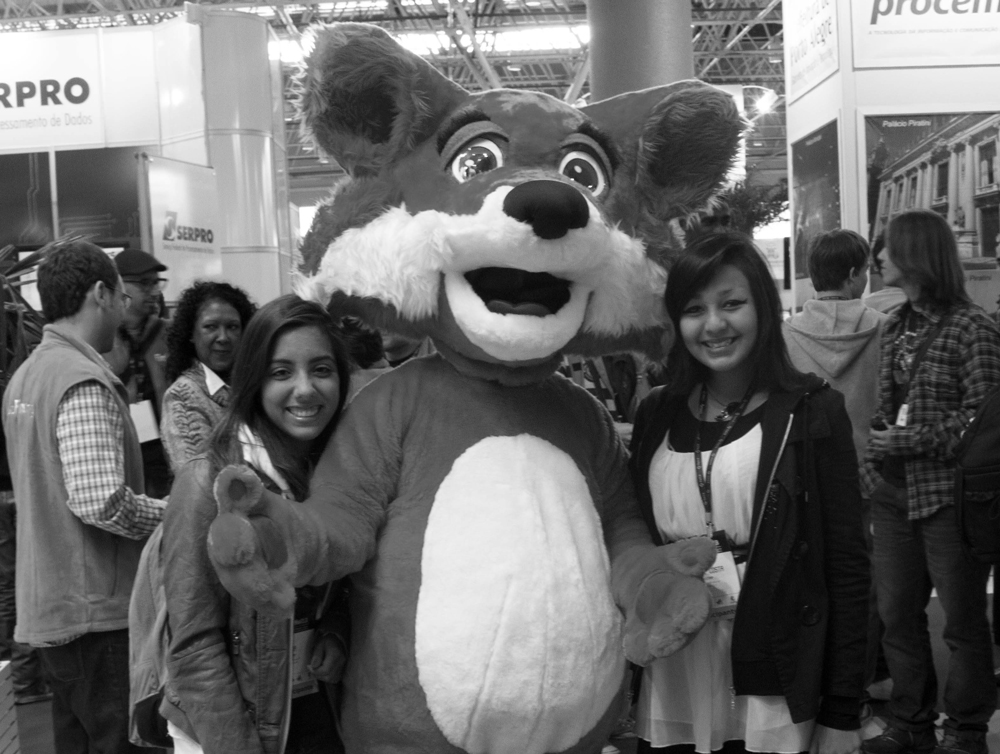
\includegraphics[scale=0.21]{img/caco/fisl.jpg}
\end{figure}

\subsection{Pesquisa Salarial}

Em 2010, com a colaboração do diretor do IC, o professor Hans Liesenberg,
e da rede social Reunion, promovemos uma pesquisa salarial com
ex-alunos de computação, que ajudou a fornecer um bom panorama da realidade em que se encontra
o profissional formado pela Unicamp na área de computação. A pesquisa
está disponível no site do CACo.

\subsection{CineCACo}

Por que não juntar com a galera no IC para assistir um filme com pipoca e
refriegerante de graça?

\subsection{PipoCACo}

Os PipoCACos são eventos de discussão sobre assuntos polêmicos, mas sem
comentários sobre  mamilos. Trata-se de um espaço para que toda a Computação
possa discutir um assunto de interesse geral. Por exemplo, já realizamos
PipoCACos sobre cotas em universidades públicas, sobre o Enade e semestralmente fazemos o PipoCACo de
Avaliação de Curso, onde reunimos as reclamações dos alunos para a reunião de
avaliação. Além de um ótimo local para ouvir opiniões e debater, os PipoCACos
são regados a refrigerante e pipoca por nossa conta!

\subsection{Palestra Azoide/Bzoide}

Chega um momento na vida de todo computeiro engenheiro em que ele deve responder
às questões fundamentais como: De onde viemos? Para onde vamos? Onde vamos
almoçar hoje? Vou ser Azoide ou Bzoide?

O curso de Engenharia de Computação da Unicamp se divide em duas habilitações, também conhecidas como modalidades: AA
e AB. A diferença? Não é simples! Por isso, o CACo organiza uma série de
palestras a fim de ajudá-lo a escolher a modalidade que mais lhe agrada.

\subsection{CACo Series of Poker}

O lendário torneio de Poker do CACo. Aberto a toda a computação, o CSoP é um
ótimo evento de integração e já contou com cinco edições de absoluto sucesso!
Você será informado da data do próximo, fique ligado!

\begin{figure}[H]
    \centering
    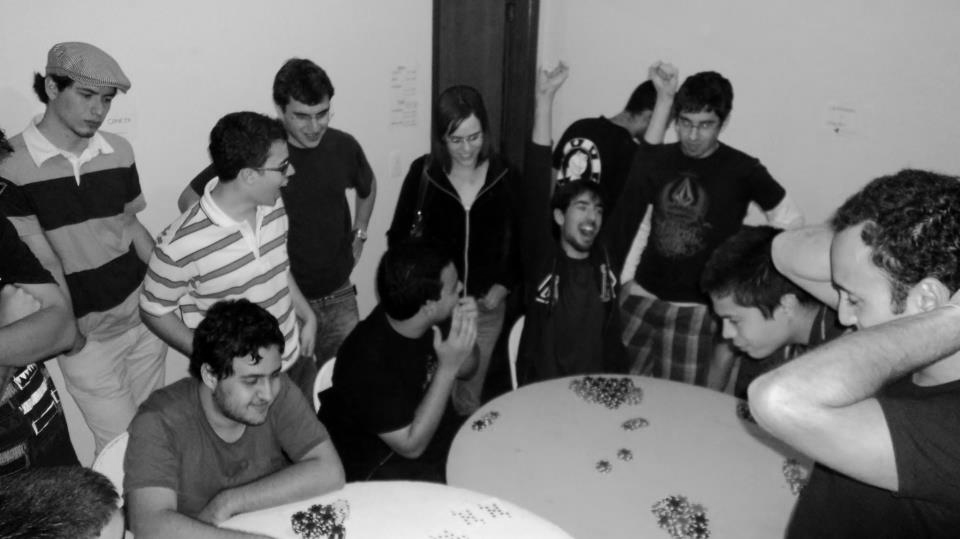
\includegraphics[scale=0.21]{img/caco/poker2.jpg}
\end{figure}

\subsection{Salinha}

A sede do CACo fica na nossa salinha no IC-3. Munida de uma incrível mesa de
sinuca, ela está aberta 24/7 para todos os computeiros que queiram jogar.

\subsection{Atendimento}

O CACo realiza atendimentos na nossa salinha. Nesses horários, você poderá
comprar nossos produtos, se inscrever em algum de nossos eventos ou só bater papo
com a gente mesmo. Os horários de atendimento serão divulgados no início do
semestre e você pode conferi-los no site do CACo.

\begin{figure}[H]
    \centering
    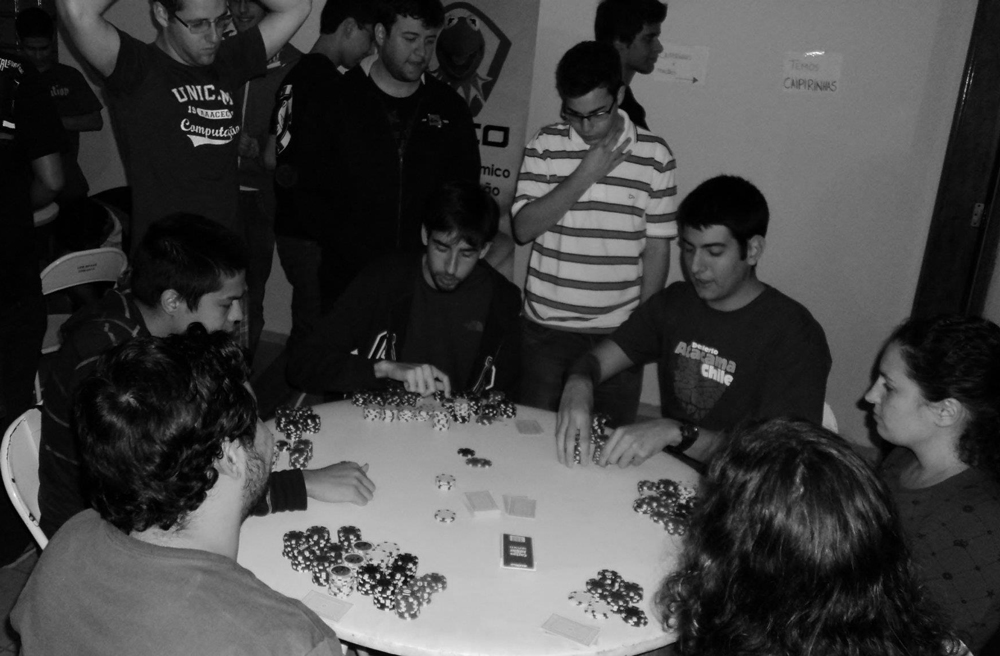
\includegraphics[scale=0.21]{img/caco/poker.jpg}
\end{figure}

\subsection{Gestão}

O CACo tem uma gestão composta de gente bonita e charmosa. Não se preocupe, se
você não é bonito nem charmoso, você ainda pode entrar na gestão... talvez. A
atual gestão foi eleita em novembro de 2012 e deve permanecer até outubro de
2013. Mas não pense que só a gestão gere o CACo. Mais uma vez: o CACo é o seu
centro acadêmico. Você e toda a computação também fazem parte do CACo e têm papel
nas nossas decisões e discussões.

Para ficar mais integrado ao que ocorre no seu centro acadêmico, como suas
ações, projetos e quais os problemas atuais, você pode se increver na lista do
CACo no Google Groups por meio do link:
\url{groups.google.com/group/cacounicamp}.

\begin{figure}[H]
    \centering
    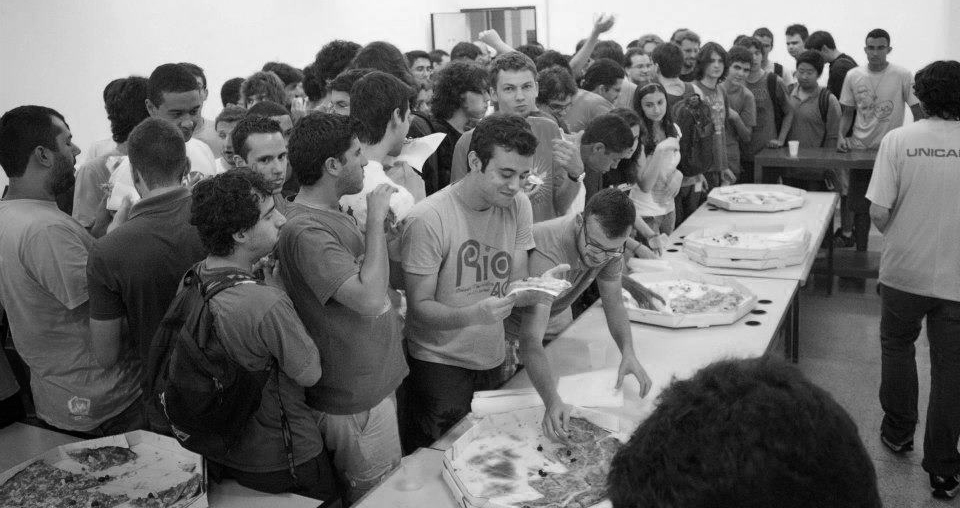
\includegraphics[scale=0.21]{img/caco/pizzada2.jpg}
\end{figure}

\begin{figure}[H]
    \centering
    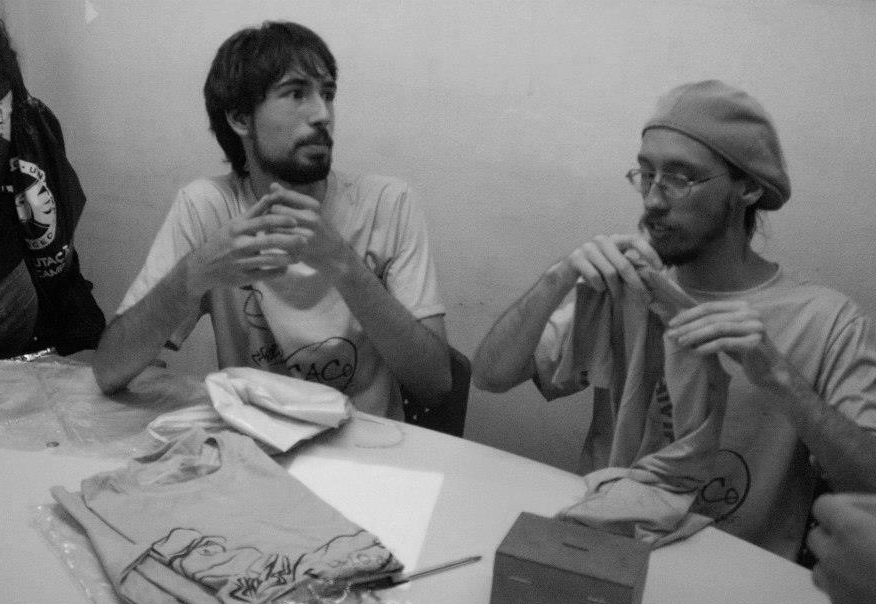
\includegraphics[scale=0.24]{img/caco/eleicao.jpg}
\end{figure}

\subsubsection{Chapa ``CACoCota'' (2012/2013)}

\begin{itemize}
\item   \textbf{Presidência}
		\\Julia Ramos Beltrão (Julia EC011)

\item   \textbf{Coordenadoria Administrativa}
		\\Alexandre Novais de Medeiros (Salsicha CC011)
		\\Victor Rodrigues Matsuguma (Preciso EC011)

\item   \textbf{Coodenadoria Financeira}
		\\Gabriel Militão Vinhas Lopes (Gagau EC012)
		\\André Felipe Barros Selva (Selva EC09)
		\\Guilherme Bueno Andrade (Laika EC012)

\item   \textbf{Coordenadoria de Ensino e Graduação}
		\\Pedro Henrique Azevedo Amorim (Amorim EC011)
		\\Brunno Rodrigues Arangues (Brunno EC010)

\item   \textbf{Coordenadoria de Ensino e Pós-Graduação}
		\\Eric Velten de Melo (Eric EC07)

\item   \textbf{Coordenadoria de Comunicação}
		\\Pedro Cordeiro de Almeida (Pedroka CC012)
		\\Yuri Corrêa Pinto Soares (Yuri CC012)
		\\Gérson de Paulo Carlos (Gérson EC09)

\item   \textbf{Coordenadoria de Eventos e Cultura}
		\\Antonio José Pinheiro Prado (Alegria EC012)
		\\Murilo Vieira Santa Bárbara (Buxexa EC012)
		\\Wesley Marques Dias (Kiabbo EC010)
		\\Humberto Aboud Torres Lobo (Sheldon EC010)
		\\Gustavo Menezes Rocha (Espanhol EC011)
		\\William Hideki Azana Tustumi (William EC011)

\item   \textbf{Coordenadoria de Marketing}
		\\Matheus Jun Ota (Ota CC012)
		\\Gabriel Rolfsen Franzoni (Clits EC012)
		\\Thiago Rosario Caetano (Thiago EC010)
		\\Jucélio Evangelista Fonseca (Jeff CC012)

\item   \textbf{Coordenadoria de Produtos}
		\\Hugo Aboud Torres Lobo (Hugo EC012)
		\\José Américo Nabuco Leva Ferreira de Freitas (Jota EC010)

\item   \textbf{Coordenadoria Tecnológica}
		\\Gabriel Hidasy Rezende (Sam EC011)
		\\Gustavo de Mello Crivelli (Jobs EC012)
		\\Matheus Mostiack Pomaleski (Poma EC011)
		\\Pedro Emílio Machado de Brito (Asmina EC012)

\end{itemize}

As gestões dos anos anteriores podem ser vistas no site do CACo.

\begin{figure}[H]
    \centering
    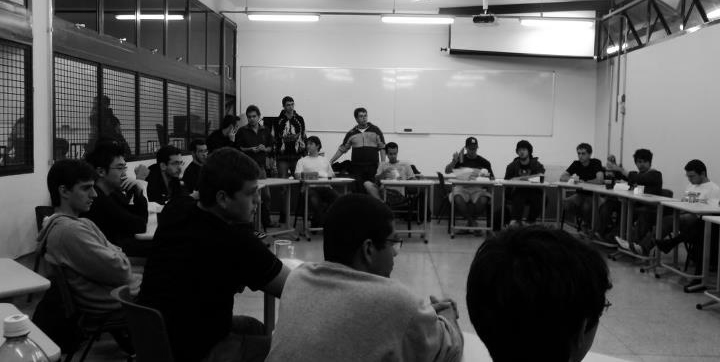
\includegraphics[scale=0.29]{img/caco/pipocaco.jpg}
\end{figure}
